\section{Introducción}

En la última década, la incorporación de Tecnologías de la Información en los entornos rurales ha dejado de ser considerada un simple valor agregado opcional para constituirse en un requisito indispensable de supervivencia comercial y competitividad sistémica. En el contexto geopolítico y económico del departamento del Huila, Colombia, se evidencia una brecha histórica de carácter paradójico: la región ostenta una producción agrícola de alta calidad —reconocida nacional e internacionalmente en rubros de alta demanda como el café especial, el cacao y las frutas exóticas—, pero carece de la infraestructura digital necesaria para visibilizarla de forma efectiva ante los mercados globales.

Esta desconexión genera una profunda asimetría de información. Mientras el mercado final demanda trazabilidad y origen, el productor primario, quien es el verdadero generador del valor económico, queda relegado al eslabón más débil de la cadena de suministro, dependiendo de intermediarios que capturan la mayor parte del margen de rentabilidad. Como sostienen \cite{garcia2007informacion}, la sostenibilidad de cualquier organización compleja —incluidas las redes de pequeños productores agrícolas y las cooperativas rurales— depende intrínsecamente de su capacidad para gestionar, procesar y capitalizar el conocimiento. Si la información no fluye con la misma velocidad que el producto físico, el negocio se estanca.

Bajo esta premisa surgió la iniciativa del Portal Agro-Comercial, concebido no solo como un sitio web informativo o un catálogo estático, sino como una solución tecnológica estratégica diseñada para conectar a las fincas del municipio de Teruel directamente con los compradores finales. El objetivo explícito es eliminar las capas de intermediación ineficientes y devolver el control del precio y la negociación al productor.

% --- INICIO FIGURA: Brecha Digital ---
\begin{figure}[htbp]
    \centering
    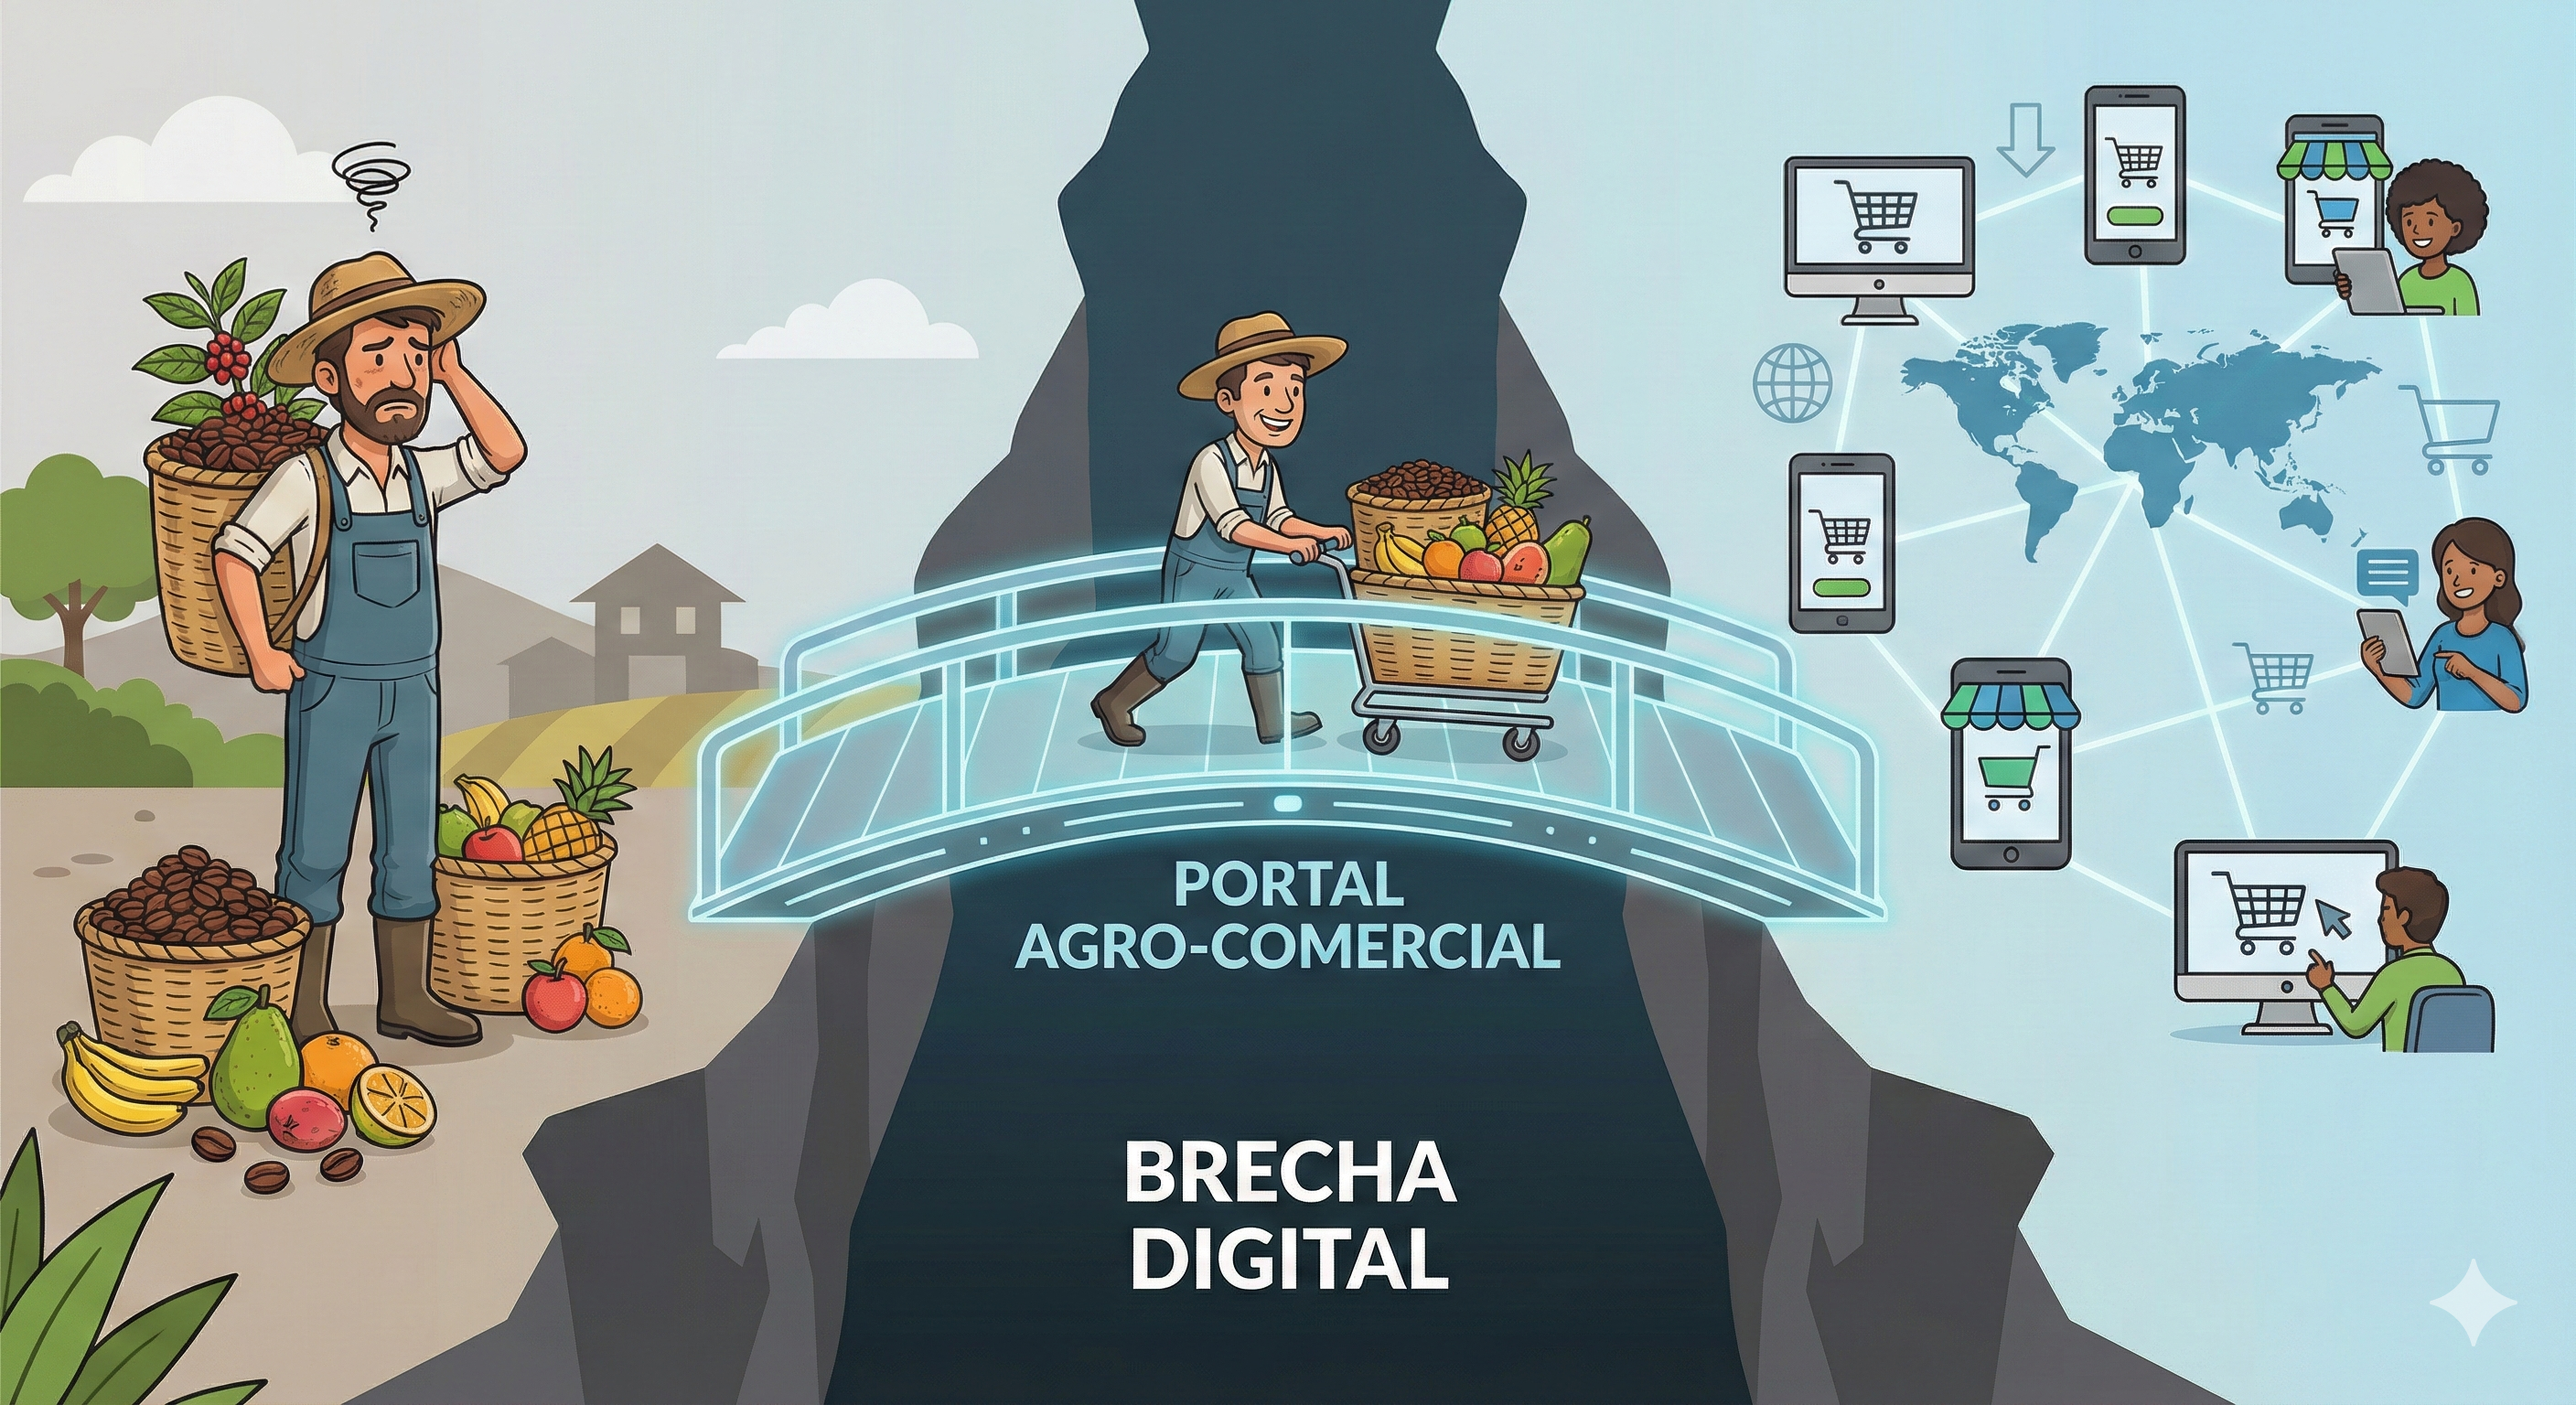
\includegraphics[width=0.85\columnwidth]{graphics/brecha_digital_agro.png}
    \caption{Ilustración conceptual de la brecha entre la producción agrícola de alta calidad y su limitada visibilidad en el mercado digital, mostrando cómo el Portal Agro-Comercial actúa como un puente tecnológico.}
    \label{fig:brecha_digital}
\end{figure}
% --- FIN FIGURA ---

En su fase constructiva inicial, el desarrollo del portal se adhirió al paradigma clásico de la ingeniería de software. Se ejecutó un ciclo de vida de desarrollo (SDLC) estándar, priorizando la captura de requisitos funcionales que permitieron desplegar un Producto Mínimo Viable (MVP) exitoso: un catálogo de productos, un sistema de gestión de usuarios y la generación de identidad digital para las fincas. Sin embargo, la transición desde un entorno de desarrollo controlado hacia la operación en contextos reales —con usuarios no nativos digitales y condiciones de conectividad fluctuantes— reveló con rapidez las limitaciones estructurales de este enfoque tradicional.

El problema central radica en la arquitectura de despliegue monolítica. A medida que el sistema escala y los agricultores demandan nuevas funcionalidades más sofisticadas (como reportes climáticos locales, integración con pasarelas de pago o precios de referencia en tiempo real), los modelos de despliegue tradicionales se convierten en un cuello de botella operativo. En el modelo actual, un simple \textit{hotfix} obliga a detener el servicio, reemplazar los binarios y reiniciar la aplicación completa.

Esta rigidez arquitectónica resulta crítica por dos razones. Primero, interrumpe la operación comercial; en un entorno digital que opera 24/7, cada caída del sistema implica ventas perdidas. Segundo, y aún más grave, erosiona la confianza del usuario. Cuando los agricultores dependen de esta herramienta para concretar transacciones diarias, cualquier inestabilidad genera una resistencia al cambio tecnológico difícil de revertir. La industria del software reconoce este problema, y por ello el paradigma de la Entrega Continua (\textit{Continuous Delivery}), analizado empíricamente por \cite{meyer2016continuous}, se consolida como la vía necesaria para eliminar el temor a “romper el sistema” en cada actualización.

Es en este punto donde las \textit{Feature Toggles} (también denominadas \textit{feature flags}) emergen como un componente arquitectónico esencial. Más allá de una simple técnica de programación condicional, \cite{rahman2016msr} las definen como una estrategia que permite alterar el comportamiento del software en tiempo de ejecución sin modificar el código compilado ni interrumpir el servicio.

Aunque el Portal Agro-Comercial no fue concebido originalmente bajo este paradigma, un análisis estructural profundo evidencia que constituye un candidato idóneo para esta transición. La incorporación de toggles permitiría habilitar escenarios de validación progresiva en producción, donde nuevas funcionalidades se prueban con subconjuntos de usuarios antes de su liberación masiva.

La literatura reciente respalda esta dirección. Estudios como los de \cite{garcia2021practitioners} demuestran que los toggles no solo introducen beneficios técnicos, sino que transforman la cultura de los equipos de desarrollo al permitir separar dos procesos históricamente acoplados: el **despliegue** (instalación del código en servidores) y la **liberación** (activación de funcionalidades al usuario). Esta distinción resulta crítica para proyectos con soporte técnico limitado y alto impacto reputacional ante fallos en producción.

No obstante, esta transición no está exenta de riesgos. La inyección sistemática de lógica condicional introduce desafíos de calidad de software. Investigaciones recientes, como las de \cite{sharma2024complexity}, evidencian una correlación directa entre la proliferación de toggles y el aumento de la complejidad ciclomática. Si esta lógica no se gobierna mediante políticas estrictas de control y eliminación de deuda técnica, el código puede degradarse en mantenibilidad, dificultando las pruebas, la depuración y la evolución futura.

En consecuencia, este artículo persigue dos objetivos complementarios. Primero, documentar con rigor la experiencia constructiva del Portal Agro-Comercial como un caso de estudio real de digitalización rural en Colombia, exponiendo con transparencia sus logros funcionales y sus debilidades arquitectónicas. Segundo, proponer y modelar un esquema robusto de implementación de \textit{Feature Toggles}, fundamentado en una revisión sistemática de 20 artículos especializados. Se busca demostrar que la adopción controlada de esta técnica constituye una respuesta efectiva a los problemas de escalabilidad y deuda técnica, permitiendo que la plataforma evolucione de forma sostenible sin colapsar ante su propio crecimiento.
